%
\section{Practical foundations}
\label{sec_3}

After the formal and logical foundations this chapter introduces
the practical aspects of building and using such a logic to build
reliable distributed systems is presented. This section covers Raft,
a state of the art protocol to build distributed systems.
Afterwards, a way to additionally harden such systems by using
the \textit{proofs-as-programs} approach is described.
This includes a short explenation of \textit{COQ} as well as
\textit{Velisarios} which is used to implement the \textit{RAFT}
consensus protocol.

\subsection{Consensus Algorithms}
As mentioned in the introduction, distributed systems are useful to harden
critical infrastructures. A critical infrastructure is one where failures
of single components could lead to a desaster. So the informations and
actions of single components shall be distributed and replicated to multiple
components holding the same state. The distributed system manages a
global state which is replicated over multiple members of the system and
a failure of some members can be tolerated. To harden the system further
the definition of failure is slightly different.~\cite{rahli2018velisarios}

\begin{defi}
  A byzantine failure is a failure which imposes no conditions.
\end{defi}

This means that a failure could happen at any time and the distributed
system has no relaible way to detect that a member failed or is malfunctioning.
Furthermore, a member could distribute false informations across the network
and the system has to react reliable consistent to a certain limit a failures.~\cite{lamport1982byzantine}

\begin{defi}
  A typical byzantine fault-tolerant system can tolerate $n=3f+1$ failures
  where $n$ gives the amount of members in the network to tolerate $f$ byzantine
  members.
\end{defi}

\begin{defi}
  A consensus protocol is an algorithm that allows a network of machines to
  agree on a common state of the network. The members act as a coherent
  group which could tolerate failures of individual members.
\end{defi}

A consensus protocol is a state-of-the-art approach to build reliable and
resilent distributed systems which can tolerate byzantine failures.

\begin{figure}[ht]
  \centering
  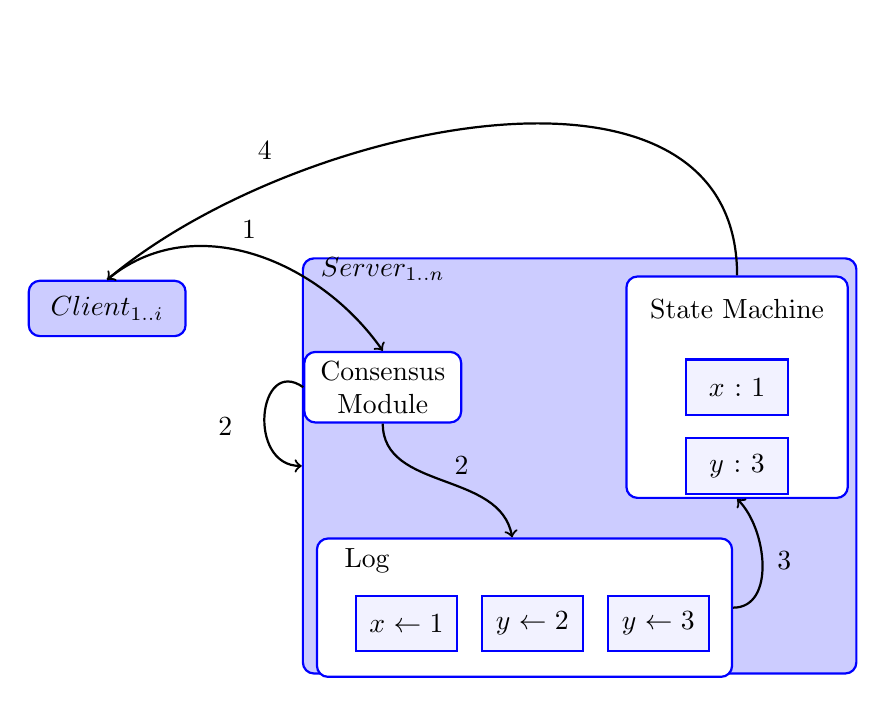
\begin{tikzpicture}[
    auto,
    block/.style={
      rectangle,
      draw=blue,
      thick,
      fill=blue!20,
      text width=5em,
      align=center,
      rounded corners,
      minimum height=2em
    }]

    % client box
    \draw (-6,2) node[block] (C) {$Client_{1..i}$};
    % server box
    \draw (0,0) node[
    block,
    minimum height=15em,
    minimum width=20em] (N) {};
    \node at (-2.5,2.5) {$Server_{1..n}$};
    % consensus
    \draw (-2.5,1) node[block,fill=white] (M) {Consensus Module};
    % log
    \draw (-0.7,-1.8) node[
    block,
    fill=white,
    minimum width=15em,
    minimum height=5em] (L) {};
    \node at (-2.7,-1.2) {Log};
    \draw (-2.2,-2) node[block,fill=blue!5,sharp corners,text width=3em] {$x\leftarrow 1$};
    \draw (-0.6,-2) node[block,fill=blue!5,sharp corners,text width=3em] {$y\leftarrow 2$};
    \draw (1,-2) node[block,fill=blue!5,sharp corners,text width=3em] {$y\leftarrow 3$};

    % state machine
    \draw (2,1) node[
    block,
    fill=white,
    minimum height=8em,
    minimum width=8em] (S) {};
    \node at (2,2) {State Machine};
    \draw (2,1) node[block,fill=blue!5,sharp corners,text width=3em] {$x: 1$};
    \draw (2,0) node[block,fill=blue!5,sharp corners,text width=3em] {$y: 3$};

    % lines
    \draw[->, thick] (C.north) to[out=40,in=125] (M.north) node at (-4.2,3) {1};
    \draw[->, thick] (M.south) to[out=-90,in=100] (L) node at (-1.5,0) {2};
    \draw[->, thick] (M.west) to[out=145,in=180,distance=2em] (N.west) node at (-4.5,0.5) {2};
    \draw[->, thick] (L.east) to[out=0,in=-45] (S.south) node at (2.6,-1.2) {3};
    \draw[->, thick] (S.north) to[out=90,in=40] (C.north) node at (-4,4) {4};
  \end{tikzpicture}
  \caption{Overview of the replicated state machine architecture.~\cite{ongaro2014search}}
  \label{fig:pbftsm}
\end{figure}

In figure~\ref{fig:pbftsm} an overview of the generic structures of the
replicated state machine architecture is presented. Most protocols using
replicated state machines act in the same manner. A possible bunch of clients
send their requests to the distributed network (1). The network can consist
of multiple servers. The consensus module is the middleware implementation of
the consensus protocol and acts as mediator between the clients and servers.
The request is forwarded to all server consensus modules within the network (2).
Also the request is added to the server log. The request is seen as a command to
the server state machine and gets applied if the majority of the network
recieved the new command (3). Afterwards, the client recieves the result (4).
All server logs contain the same commands in the same order. So the servers
state machines process the commands in the same order and produce the same output.~\cite{ongaro2014search}

The major parts of the consensus algorithm are to ensure that the logs are
consistent across the servers, to manage the client network communication,
handle the replication across the network and keep the network alive if
some server fails. So a consensus algorithm ensures the following properties:~\cite{ongaro2014search}

\begin{itemize}
\item Ensure safty under all non-Byzantine conditions.
\item Ensure availability as long as the majority of servers is
  functional and can communicate.
\item Consistency doesn't depend on timing.
\item The system performance depends on the majority of servers
  and minarities can be ignored.
\end{itemize}

One early approach to build such distributed systems was presented by
Leslie Lamport et al as Paxos in~\cite{lamport1978time}.
Most of the newer protocols are directly derived from the early Paxos
protocol like~\cite{lamport2001paxos, van2015paxos}.
As Ongaro et al stated in~\cite{ongaro2014search} the family of
Paxos protocols suffer from two problems. Besides they ensure the
properties and provide a efficent protocol, the protocols are
difficult to understand. The descriptions are ``notoriously
opaque''~\cite{ongaro2014search} and are mostly focused on a
subset of the real world protocol. The other problem is that the
most descriptions are not implementation ready and a huge effort
is needed to complete the missing parts of the protocol.
So, real implementation reflect the paxos protocol only at
the beginning. To tackle these problems Ongaro et al made
the effort to design a new consensus protocol without the
Paxos history. This new protocol RAFT was designed with
understandability in mind. This means, that the implementers
effort needs to be minimized and the description and pseudo-code
needs to be as close to the real world as possible. Also,
the properties mentioned before needs to be taken into account.
The resulting protocol shall be efficient and safe under
typical conditions and operations.~\cite{ongaro2014search}



\subsubsection*{The RAFT protocol}
The algorithm is designed to manage a replicated log
across a distributed network. The protocol uses a leader-based
approach where one distinguished leader takes the full responsibility
for log replication and client handling. The other nodes are
only serving as replicas without own intentions. This approach
leads to a three main components which can be viewed quite separated.~\cite{ongaro2014search}

\begin{itemize}
\item Leader election: Elect a new leader if the existing leader fails.
\item Log replication: The leader manages client requests and takes care
  of replicating his log across the network.
\item Safety:  The key property is the state machine safety which means that
  if any server has applied a log entry no other server applies a
  different log entry at the same log index.
\end{itemize}

The last point is a set of five properties to ensure the liveness and
safety of the Raft protocol. The individual points are discussed at
their belongings.~\cite{ongaro2014search}

\begin{itemize}
\item Election safety: At all times at most one leader can be elected.
\item Leader Append-Only: New entries are only appended to the log and
  a leader never overwrites or deletes entries from it's log.
\item Log Matching: If an entry is contained in two logs with the same
  term and index, these logs are identical up til the entries index.
\item Leader Completness: If an entry is committed in some term, then the
  entry is present in all leader logs in all higher terms.
\item State Machine Safety: If an log entry with some index is applied to
  the internal state machine, then no other server ever applies a
  different log entry at the same index.
\end{itemize}

\paragraph{Basics}
A consensus protocol doesn't use real time to measure the protocol progress
instead the time is divided into abstracts chunks of time. These chunks
serve as the logical clock of the protocol.~\cite{ongaro2014search}

\begin{defi}
  Time is divided into terms of arbitrary length where each term
  starts with an election phase which can be followed by a normal
  operation phase.
\end{defi}

This can be seen in figure~\ref{fig:terms}. The first term starts with an
election phase followed by a normal operation phase. The leader fails and
the term ends. The next terms starts with an election phase which results in no
new leader and the next term is started.
Terms are numbered by consecutive integers and servers may observe term
transitions at different times. Each server stores it current term number
and exchanges it at every communication to detect failed leaders or outdated
data.~\cite{ongaro2014search}

\begin{figure}[ht]
  \centering
  \begin{tikzpicture}[>=stealth',shorten >=1pt,auto,node distance=4cm,semithick]

    \draw[->] (-5,0) -- (5,0) node at (5,-0.5) {terms};
    % first term
    \draw (-4,0.5) -- (-4,-0.5);
    \draw (-3,0.5) -- (-3,-0.5);
    \draw (-1.5,0.5) -- (-1.5,-0.5);
    \draw[decoration={brace,mirror,raise=5pt},decorate] (-4,-0.5) -- node[below=12pt] {$term_1$} (-1.5,-0.5);
    \draw[decoration={brace,raise=5pt},decorate] (-4,0.5) -- node[above=8pt] {\scriptsize$election$} (-3,0.5);
    \draw[decoration={brace,raise=5pt},decorate] (-3,0.5) -- node[above=15pt] {\scriptsize$normal\ operation$} (-1.5,0.5);


    % second term
    \draw (-0.5,0.5) -- (-0.5,-0.5);
    \draw (0.5,0.5) -- (0.5,-0.5);
    \draw[decoration={brace,mirror,raise=5pt},decorate] (-0.5,-0.5) -- node[below=12pt] {$term_2$} (0.5,-0.5);
    \draw[decoration={brace,raise=5pt},decorate] (-0.5,0.5) -- node[above=8pt] {\scriptsize$split\ vote$} (0.5,0.5);

    %third term
    \draw (4,0.5) -- (4,-0.5);
    \draw (2,0.5) -- (2,-0.5);
    \draw (1.5,0.5) -- (1.5,-0.5);
    \draw[decoration={brace,mirror,raise=5pt},decorate] (1.5,-0.5) -- node[below=12pt] {$term_3$} (4,-0.5);
    \draw[decoration={brace,raise=5pt},decorate] (1.5,0.5) -- node[above=8pt] {\scriptsize$election$} (2,0.5);
    \draw[decoration={brace,raise=5pt},decorate] (2,0.5) -- node[above=15pt] {\scriptsize$normal\ operation$} (4,0.5);

  \end{tikzpicture}
  \caption{Example timeline within the protocol process.}
  \label{fig:terms}
\end{figure}

A server can be in one of three possible states at all times.
A server can either be a \textit{leader}, a \textit{follower} or a
\textit{candidate}. Figure~\ref{fig:serverstates} shows the state
and the transition between them. Only one leader is allowed in normal operation
and all other servers are passive followers which obey the leaders commands.
The followers aren't issueing requests on their own (except message forwardng to
the current leader) and only respond to requests from the leader and candidates.
The leader handles all client communication and manages log replication across
the followers. The candidate state is only entered if the leader fails and
a new leader needs to be elected.~\cite{ongaro2014search}

\begin{figure}[ht]
  \centering
  \begin{tikzpicture}[->,>=stealth',shorten >=1pt,auto,node distance=4cm,
    semithick]
    \tikzstyle{every state}=[rectangle]

    \node[initial,state] (A) {$Follower$};
    \node[state]         (B) [right of=A] {$Candidate$};
    \node[state]         (C) [right of=B] {$Leader$};

    \draw (A.north) to[out=45,in=125] (B.north west) node[align=left] at (0,1.5) {times out\\start election};
    \draw (B.north) to[out=125,in=45,distance=5em] (B.north) node[align=left] at (4,2) {times out\\new election};
    \draw (B.north east) to[out=45,in=125] (C.north) node[align=left] at (8,1.5) {recieves votes from majority};
    \draw (B.south) to[out=-125,in=-45] (A.south east) node[align=left] at (4,-3) {discovers server with higher term};
    \draw (C.south) to[out=-125,in=-45] (A.south) node[align=left] at (5,-1.5) {discovers current leader\\or new term};

  \end{tikzpicture}
  \caption{The server state transistions diagram.~\cite{ongaro2014search}}
  \label{fig:serverstates}
\end{figure}

\paragraph{Leader election}
As stated in the figure~\ref{fig:serverstates} raft uses timeouts to handle
leadership and election. Thus, every server has an internal timer with a
random time (mostly between 150 and 300ms) which gets resetted with
every message from a leader. Besides normal messages the leader uses
heartbeat messages to reset the follower timers if the cluster is idle.
If a follower recieves no messages over a period of time the
follower gets an \textit{election timeout}. It assumes the leader
failed and turns into candidate state starting a new term and
election. The election runs as follows:~\cite{ongaro2014search}

\begin{enumerate}
\item A follower times out by recieving no messages over a period of time.
\item A follower increments its current term and turns into candidate state.
\item A candidate votes for itself and issues the vote to the cluster.
\item Continue with point one until one of the follwing happens:
  \begin{enumerate}
  \item The candidate wins the election.
  \item Another candidate wins the election.
  \item The election times out with no winner.
  \end{enumerate}
\end{enumerate}

Since this maybe happens in parallel on many servers more details
need to take into account when determing the possible outcomes.

(a) A candidate wins the election when it recieves the majority of
votes in the cluster. Each server votes for one candidate on a
\textit{first-comes-first-served} basis. The majority voting ensures
the only one leader safety property. The winner imediatly starts
by sending heartbeat messages to all other servers to implement itself
as new leader and stop the election phase.~\cite{ongaro2014consensus}\\
(b) A candidat may recieve messages from a possible new leader.
The new leader is accepted if it's term is at least as large as
the candidates one. The candidate accepts the new leader and turns
into follower state. Otherwise, the leader is rejected and the election
goes on.~\cite{ongaro2014consensus}\\
(c) If multiple candidates start with the election at the same
time or the network connection is poor enough no candidate may win
the election. In this split vote scenario the candidate times out again
and starts a new term and election phase.\cite{ongaro2014consensus}

\paragraph{Log replication}
If a leader is elected the cluster transistions to the normal operation
state. This means that client requests are served, the requests are
replicated across the cluster and applied to the state machines.
The leader processes the client requests which contain commands to
the replicated state machine. The command is appended to the leaders
log as a new entry. Afterwards the leader issues replication requests
of this new entry to all other servers in parallel. If the majority
replicated the entry the leader commits the entry to it's state machine
and repsonds the results to the client. The follower are noticed by
later messages of this newly committed entry. The leader
tries the replication of an entry indefinitly if some followers
are creashed or not responding.~\cite{ongaro2014search}

Figure~\ref{fig:logs} shows the organization of the logs of five servers,
one leader and four followers. Each entry carries the command for the state
machine and the term number the entry was created to detect inconsistencies
between logs. Additionally, an entry is assigned to some log index number.
If an entry was safely replicated across the network and leader applies
it to its state machine, then the entry is committed and durable over
future terms. Also, the entry is eventually applied by all state machines
in the cluster. The leader tracks the highest known log index and includes
it in future request such that followers know which entries can be
safely applied to their state machine. Previous entries which are
not already applied are also applied in log order.~\cite{ongaro2014consensus}

\begin{figure}[ht]
  \centering
  \begin{tikzpicture}[>=stealth',shorten >=1pt,auto,node distance=4cm,semithick]

    \draw[->] (-5,0) -- (3.9,0) node at (0,-0.5) {committed entries};
    \draw[-] (-5,0.2) -- (-5,-0.2);

    % first log
    \node at (-4.4,1) [draw,thick,rectangle,align=center,minimum height=1.2cm] {$1$\\$x\leftarrow 3$};
    \node at (-3.15,1) [draw,thick,rectangle,align=center,minimum height=1.2cm] {$1$\\$y\leftarrow 1$};
    \node at (-1.9,1) [draw,thick,rectangle,align=center,minimum height=1.2cm] {$1$\\$y\leftarrow 9$};
    \node at (-0.65,1) [draw,thick,rectangle,align=center,minimum height=1.2cm] {$2$\\$x\leftarrow 2$};
    \node at (0.61,1) [draw,thick,rectangle,align=center,minimum height=1.2cm] {$3$\\$x\leftarrow 0$};
    \node at (1.87,1) [draw,thick,rectangle,align=center,minimum height=1.2cm] {$3$\\$y\leftarrow 7$};
    \node at (3.13,1) [draw,thick,rectangle,align=center,minimum height=1.2cm] {$3$\\$x\leftarrow 5$};
    % second log
    \node at (-4.4,2.5) [draw,thick,rectangle,align=center,minimum height=1.2cm] {$1$\\$x\leftarrow 3$};
    \node at (-3.15,2.5) [draw,thick,rectangle,align=center,minimum height=1.2cm] {$1$\\$y\leftarrow 1$};
    % third log
    \node at (-4.4,4) [draw,thick,rectangle,align=center,minimum height=1.2cm] {$1$\\$x\leftarrow 3$};
    \node at (-3.15,4) [draw,thick,rectangle,align=center,minimum height=1.2cm] {$1$\\$y\leftarrow 1$};
    \node at (-1.9,4) [draw,thick,rectangle,align=center,minimum height=1.2cm] {$1$\\$y\leftarrow 9$};
    \node at (-0.65,4) [draw,thick,rectangle,align=center,minimum height=1.2cm] {$2$\\$x\leftarrow 2$};
    \node at (0.61,4) [draw,thick,rectangle,align=center,minimum height=1.2cm] {$3$\\$x\leftarrow 0$};
    \node at (1.87,4) [draw,thick,rectangle,align=center,minimum height=1.2cm] {$3$\\$y\leftarrow 7$};
    \node at (3.13,4) [draw,thick,rectangle,align=center,minimum height=1.2cm] {$3$\\$x\leftarrow 5$};
    \node at (4.4,4) [draw,thick,rectangle,align=center,minimum height=1.2cm] {$3$\\$x\leftarrow 4$};
    % fourth log
    \node at (-4.4,5.5) [draw,thick,rectangle,align=center,minimum height=1.2cm] {$1$\\$x\leftarrow 3$};
    \node at (-3.15,5.5) [draw,thick,rectangle,align=center,minimum height=1.2cm] {$1$\\$y\leftarrow 1$};
    \node at (-1.9,5.5) [draw,thick,rectangle,align=center,minimum height=1.2cm] {$1$\\$y\leftarrow 9$};
    \node at (-0.65,5.5) [draw,thick,rectangle,align=center,minimum height=1.2cm] {$2$\\$x\leftarrow 2$};
    \node at (0.61,5.5) [draw,thick,rectangle,align=center,minimum height=1.2cm] {$3$\\$x\leftarrow 0$};
    % fifth log
    \node at (-4.4,7) [draw,thick,rectangle,align=center,minimum height=1.2cm] {$1$\\$x\leftarrow 3$};
    \node at (-3.15,7) [draw,thick,rectangle,align=center,minimum height=1.2cm] {$1$\\$y\leftarrow 1$};
    \node at (-1.9,7) [draw,thick,rectangle,align=center,minimum height=1.2cm] {$1$\\$y\leftarrow 9$};
    \node at (-0.65,7) [draw,thick,rectangle,align=center,minimum height=1.2cm] {$2$\\$x\leftarrow 2$};
    \node at (0.61,7) [draw,thick,rectangle,align=center,minimum height=1.2cm] {$3$\\$x\leftarrow 0$};
    \node at (1.87,7) [draw,thick,rectangle,align=center,minimum height=1.2cm] {$3$\\$y\leftarrow 7$};
    \node at (3.13,7) [draw,thick,rectangle,align=center,minimum height=1.2cm] {$3$\\$x\leftarrow 5$};
    \node at (4.4,7) [draw,thick,rectangle,align=center,minimum height=1.2cm] {$3$\\$x\leftarrow 4$};
    
    \draw[decoration={brace,mirror,raise=5pt},decorate] (5,0.3) -- node[right=15pt] {followers} (5,6);
    \node at (5,7) [right=15pt] {leader};
    \node at (5,8.5) [right=15pt] {log index};
    \node at (-4.4,8.5) {1};
    \node at (-3.15,8.5) {2};
    \node at (-1.9,8.5) {3};
    \node at (-0.65,8.5) {4};
    \node at (0.61,8.5) {5};
    \node at (1.87,8.5) {6};
    \node at (3.13,8.5) {7};
    \node at (4.4,8.5) {8};
    
  \end{tikzpicture}
  \caption{An example of logs and it's entries accross a cluster.~\cite{ongaro2014consensus}}
  \label{fig:logs}
\end{figure}

To maintain consistency between the logs Raft uses the aforementioned
log matching property which can be devided into two properties.

\begin{defi}
  If two entries have the same index and term in different logs, then
  they store the same command.
\end{defi}

\begin{defi}
  If two entries have the same index and term in different logs, then
  all preceding entries are identical in both logs.
\end{defi}

The leader organizes its own logs before distribution and logs stay
consistent over time. So, a leader doesn't change previous log index
entries and after distribution all other logs are coherent to the leaders
one. From this follows the first property. The second one follows
from the way an entry is replicated in the network. The leader
inlcudes the previous entry term and index in the message. The follower only
applies the entry if it finds the given privious term and index in its
own log. The consitency check preserves identical logs across the
network as long as no leader fails.~\cite{ongaro2014search}

If a leader crashes the log can became inconsistent through incomplete
replication. Also, this can be collected over multiple terms and
crashes of leaders and followers. A follower can have additional
or missing entries over multiple terms in regard to the current leader.
The Raft approach to handle this inconsistencies are fairly simple.
The leader forces the followers to duplicate the leaders log and
remove inconsistent entries from their own logs. 
To do so, the leader maintains a list of the next log index
which is send to a follower (initially the next empty log index of the leader). 
If the consistency check fails and the follower rejects to apply
an entry the leader decrements its next log index for the follower
and tries to replicate this entry. This happens until the leader
finds a matching entry in the follower log which removes all
succeding entries and the leader can apply its own log.~\cite{ongaro2014search}

\paragraph{Safety}
These mechnics doesn't ensure the safety under all circumstances.
For example, if a leader is elected which has a shorter log
then the leader before the new leader maybe removes already
committed entries from the network. This would break the
Leader Completness property mentioned earlier. So, Raft
uses additional mechnics to ensure the correctness of
the safety properties.~\cite{ongaro2014search}

\subparagraph{Election restriction}
To prevent nodes with an incomplete log to be elected
Raft prevents candidates in the voting process from winning
the election. In the voting process a candidate messages
to at least a majority of other nodes in the network.
The messages contains the log index and term of the candidate
and a the voter decides if the candidates log is up-to-date
enough to recieve that vote.~\cite{ongaro2014search}

\begin{defi}
  Given two logs, the one is more up-to-date which has
  either the later term as last log entry or if the terms
  are equal the highest log index. Otherwise, both logs
  can be considered as equal.
\end{defi}

\subparagraph{Committing old entries}
If a leader crashes before committing an entry on the
majority of followers the new leader needs to handle
this situation by committing the entry. Raft never commits
log entries from previous terms by counting replicas and
checking if they are the majority. If a new entry is committed
to the majority of servers the leader applies the Log Matching
property to restore log consistency across the network.
Also, the log entries keep their term number and the
leader doesn't overrides the term number as with other
approaches. Thus uncommitted log entries are only
committed indirectly by newer commits.~\cite{ongaro2014search}

\subparagraph{Follower and candidate failures}
Follower and candidate failures are fairly easy to handle.
Since all messages in Raft are idempotent the protocol
just resends all messages indefinitly until it gets
an expected result.~\cite{ongaro2014search}

\subparagraph{Client handling}
On startup clients choose a random server for
requests if the server is not the leader it rejects
the request with additional informations about the current leader.
Otherwise, the network can implement internal forwarding of client
requests to the current leader. If the leader is unavailable the
requests time out.~\cite{ongaro2014consensus}

Raft supports linearizable semantics for clients. Each request
appears to be executed once and instantaneously. This is implemented
by assigning a unique id to every requests. The network
caches every requests along with the corresponding reponse preventing
it from re-executing old requests.~\cite{ongaro2014consensus}

\vspace{2em}

This are only the basics of the Raft algorithm which are implemented
in this thesis. Furthermore, Raft provides description for log compaction,
cluster membership changes and more further optimizations to the basic
algorithms. The next main section provides more details on the
implmenetation of the protocol within the COQ proofing system.

\subsection{COQ}
COQ is an interactive proof assistant which enables users to formalize
specifications and develop programs that fullfill these pecifications.
These tools are developed for domains that require high standards in
development and verification of programs. Also, it enables computer
scientist and mathematicians to develop proofs in an expressive
higher-order logic.~\cite{the_coq_development_team_2019_2554024}
The formalism used to provide such features is the \textit{Calculus of Inductive
  Construction}. It's a language that aims to represent functional programs
in a ML language style and proofs in higher order logic (HOL).
It uses inductive definitions to represent data-structures, even infinite
ones. Based on the Curry-Howard-Isomorphism, COQ uses an approach based
on the \textit{Calculus of Construction} as logical
background or metalanguage as described in the proofs-as-programs
sections.~\cite{the_coq_development_team_2019_2554024,
  paulinmohring:hal-01094195} This subsection gives only a brief overview
for a more comprehensive introduction use the reference documentation\footnote{\url{https://coq.inria.fr/refman/index.html}}.

% The Calculus of Construction is an axiom-free typed polymorphic language which can
% represent inductive definitions. It is the underlying language for the
% Calculus of Inductive Construction. It is a pure and riched typed $\lambda$
% lambda-calculus which can describe terms and types.~\cite{paulinmohring:hal-01094195}
% The term includes the normal lambda operations, like binding, abstraction
% and application. The typing supports for instance  abstractions with
% dependent products and typing of types. These typing allows to ``sort''
% (a special COQ constant) types in universes and apply to them differently
% depending on the certain universe of objects.~\cite{paulinmohring:hal-01094195}

The Calculus of Construction is an axiom-free typed polymorphic language.
The language of COQ allows to define mathematical facts by
defining objects, like integers, sets, trees etc., and making statements
about the facts. By combining these one can write mathematical proofs.
The COQ compiler can automatically reason about the correctness of these
definitions and proofs by applying the rules of the type theorie.
Additionally COQ provides an enviroment to support the developer by
creating programs and proofs with various tools like proof search, advanced
notations etc.~\cite{paulin2011introduction}

To enable this, COQ uses a small kernel language with only a few
primitive constructions, e.\,g. functions, (co-)inductive definitions,
product types, sorts. It is a pure and riched type $\lambda$-calculus which
describes terms and types.~\cite{paulinmohring:hal-01094195}.
It provides the basic $\lambda$ operations like binding, abstraction
and application. Additionally, rules for type-checking and computation
are implemented on this level allowing the aforementioned reasoning
about the correctness.~\cite{paulin2011introduction, paulinmohring:hal-01094195}

The same language can be used to represent objects, functions, propositions
and proofs which are on the higher-level. For this, COQ provides a
rich enviroment for designing theories, proofs and programs. For instance,
this enviroment includes notations which are extensible, a tactic language,
a library system. These extension are conservative and only extend the
basic kernel in a safe manner.~\cite{paulin2011introduction}

\begin{defi}
  Every COQ object or term has a name and a type.
\end{defi}

\begin{defi}
  Types are building an infinite well-founded hierarchy.
  The type of types is called sort and the main sorts are:
  \begin{itemize}
  \item $Prop$ as the type of logical propositions.
  \item $SProp$ as the type of strict propositions.
  \item $Set$ as the type of small sets, for instance data types.
  \end{itemize}~\cite{the_coq_development_team_2019_2554024}
\end{defi}

\begin{defi}
  To support abstraction COQ uses \textbf{Definitions} to instantiate
  general statements with more concrete concepts used for proofs
  or programming.~\cite{huet1997coq}
\end{defi}

Definitions are one of the basic constructs which are used exentensivly
to define functions and facts about the program or theory.
Another important construct are inductive types which are used to model
data-types, primitive relations and so on in a constructive way.~\cite{paulin2011introduction}

\begin{defi}
  An inductive type declares a set of constructors which are used
  to construct every possible entity of the type. It introduces
  a new primitive object for the type and provides induction support
  on that type for reasoning.~\cite{paulin2011introduction}
\end{defi}

To use inductive types in functions or some other definitions COQ
uses \textit{pattern-matching} for case analysis over the type
constructors. It provides a strong support for this by allowing
to match multiple patterns at once or by nesting patterns which
is also called \textit{generalized
  pattern-matching}.~\cite{paulin2011introduction}

The last important syntactically point mentioned here is the \textit{fixpoint definition}
which allows to build recursive functions. To keep the logic sound, COQ uses
structural recursion instead of general recursion. This means that
such a definitions uses an inductive type as formal argument.
Thus, on a recursive call the compiler can check that the next
term is structurally smaller then the previous one.~\cite{paulin2011introduction}

\paragraph{Extraction}
To use the logical and functional programs in the real-world in conjunction
with other non-proofen or type-checked languages, COQ offers
the possibillity to extract formal code from Calculus of Inductive Construction.
The COQ objects can be extracted into either Haskell or OCaml code and
some objects also can be exchanged by efficient ones from the target
language. This thesis extracts the code as OCaml library which can be
embedded in a command-line interface or simulation or evaluation
code for the Raft protocol.~\cite{the_coq_development_team_2019_2554024}

This is only a small overview of the possibillities COQ offers. Since,
this thesis has no focus on building proofs this part was skipped and
only the basic elements for building functional programs are shown to
basically understand the Velisarios framework. Other constructs
are explained as they appear in the thesis.


\subsection{Velisarios}
This chapter showed the Raft protocols and the difficulties of
implementing distributed systems. The Logic of Events from the former
chapter shows a formal approach to handle this difficulties in
a consistnt theorie. It can tolerate byzantine-failures and
imperfect informations about the network. Rahli et al. presented
an implementation of the Logic of Events first in the NUPRL
theorem prover named EventML~\cite{rahli2017eventml}. Later
the system was reimplmented in COQ as Velisarios~\cite{rahli2018velisarios}.
It aims to be a generic and extensible formal verification framework
for developing and systematically proofing distributed networks.~\cite{rahli2018velisarios}

Schematically all byzantine fault-tolerant (BFT) protocols share the same
higher logic of distributing, gathering and voting on knowledge
provided to the system. Velisarios is a knowledge theory which
helps to build such systems by providing many main components
to reason about BFT protocols. For instance, a basic model
of the idea of arbitrary faults, a collection of assumptions
for reasoning, proof tactics and a general library of
knowledge of distributed systems.~\cite{rahli2018velisarios}

\begin{figure}[ht]
  \centering
  \begin{tikzpicture}[>=stealth',shorten >=1pt,auto, line width=1mm,semithick]

    % background layer
    \draw (0,0) node[rectangle, fill=gray!5, minimum width=10cm, minimum height=5cm] {};
    \draw (-7,0) node[rectangle, fill=gray!5, minimum width=2cm, minimum height=5cm] {};
    \draw (-7,2) node {OCaml};
    \draw (-4,2) node {COQ};

    % second layer
    \draw (-7,-0.3) node[rectangle, fill=magenta!10, rotate=-90, minimum height=1.5cm] (A) {Extraction/Execution};
    \draw (-2,0.4) node[rectangle, fill=magenta!5, minimum height=2.5cm, minimum width=5cm] {};
    \draw (-2,-1.5) node[rectangle, fill=magenta!10, minimum width=5cm] (B) {Process/State Machines};
    \draw (-4,1.3) node {LoE};
    \draw (2,0) node[rectangle, fill=magenta!10, rotate=-90, minimum height=1.5cm, minimum width=3cm] (C) {Assumption};
    \draw (4,0) node[rectangle, fill=magenta!10, rotate=-90, minimum height=1.5cm, minimum width=4.5cm] (D) {Safety Proofs};

    % top layer
    \draw (-2.6,1) node[rectangle, fill=magenta!10, minimum height=1cm, minimum width=1.5cm] (E) {Auth.};
    \draw (-2.6,-0.2) node[rectangle, fill=magenta!10, minimum height=1cm,minimum width=1.5cm] (F) {Msg};
    \draw (-0.6,0.4) node[rectangle, fill=magenta!10, align=center, minimum height=2.2cm] (G) {Event\\Orderings};

    % lines
    \draw[->] (B.west) -- (A);
    \draw[->] (E) -- (G);
    \draw[->] (F) -- (G);
    \draw[->] (B.east) -- (C);
    \draw[->] (G) -- (C);
    \draw[->] (G.45) -- (D.-160);
    \draw[->] (C) -- (D);
    \draw[->] (B.east) -- (D.-20);

    % parts
    \draw[dashed] (-5.5,3) -- (-5.5,-3) node [left] {Runtime};
    \draw[dashed] (1,3) -- (1,-3) node [left,xshift=-1.5cm] {Implementation}
    node [right] {Proofing};
    
  \end{tikzpicture}
  \caption{Overview of the Velisarios components.~\cite{rahli2018velisarios}}
  \label{fig:velisarios}
\end{figure}

As stated in the former chapter an event is an abstract entity which handles
recieved messages or reacts to some abstract activity which is no further
described. Velisarios use these arbitrary events to describe arbitrary faults.
A process reacts to messages happening at their locations one after another
by going through their states and creating new messages (which in turn
is a new event). Since events can be ordered by space and time a collection
of these events can be seen as a run of a distributed systems. These are
called \textit{event orderings}. These orderings are the main idea when proving
properties about a distributed systems.~\cite{rahli2018velisarios}

\begin{defi}
  A property $P$ holds for a distributed system if it holds
  for all event orderings of that system.
\end{defi}

Figure~\ref{fig:velisarios} shows an overview of the components provided
by Velisarios. All components are abstract and parametrized to enable
reasoning and implementation of different protocols.~\cite{rahli2018velisarios}

As one can see, the core of Velisarios is the implementation of the Logic of
Events in terms of a message and authentication model which form
the event orderings model.~\cite{rahli2018velisarios}

\paragraph*{Messages}
The messages are modeled as a type parameter \code{msg} of the overall model.
Processes react to incomming messages and may produce outgoing messages.
Basically, messages are directed which hold the destination along with
the message and and optional delay that holds the message back.~\cite{rahli2018velisarios}

\paragraph*{Destination}
A destination or node in the network has a type \code{name} which
identifies is in the network. The type belongs to the overall model.~\cite{rahli2018velisarios}

\paragraph*{Authentication}
Velisarios adds the abstract concept of keys for authenticated communication
to the overall model. A message can be authenticated by some nodes key
and the message can be checked for validity by some other node. The keys
are distinguished into sending and recieving ones which are preshared.
The model uses tokens to provide an abstraction for digital signatures.
The tokens are created by the appropriate sending key along with the data.
The recievers verifies the correctnes by checking that token with the recieving
key.~\cite{rahli2018velisarios}

This components form the event ordering component. It can be seen
as an abstract and formal representation of a run of a distributed system.
It is derived from the message sequence diagram used by most system designers.
The event orderings are no concrete type and are only used by velisarios
to prove certain properties of the distributed system.~\cite{rahli2018velisarios}

\paragraph{Computational Model}
As shown below in the figure, Velisarios provides a process or state machine
model as computational model for the logic of events. These state machines
are directly executable and the \code{name} of a node maps to the nodes
state machines. This enables the system to associate different state machines
to different nodes which can run independently.
The state machine is designed in a classical manner where
it consists out of an initial state, a current state and an update function
for state transitions as seen in Listing~\ref{lst:statemachines}.

\begin{lstlisting}[style=coq,float,label=lst:statemachines,caption=State
machine definition and update function.]
Definition Update S I O := S -> I -> (option S * O).
Record StateMachine S I O := 
  MkSM {halted : bool; update : Update S I O; state : S}.
Definition System (F : name -> Type) I O :=
  forall (i : name), StateMachine (F i) I O.
\end{lstlisting}

\code{S} is the type of the state machine and \code{I,O} are the input
and output types. The \code{halted} flag indicates if the particular
state machine is running or not. If an event \code{e} is recieved by
a state machine the local history of events is unrolled and
\code{state\_sm\_before\_event} creates the current state until
the new event. \code{state\_sm\_after\_event} updates the current
state by processing the messages of that event. Both functions
return \code{Some state} if event is processed and otherwise
\code{None} if the state machines is halted or some error occoured.~\cite{rahli2018velisarios}

\paragraph{Extraction}
To evaluate and run the implemented protocol Velisarios
uses the COQ mechanics to extract OcCaml code. Most of
the needed parameter are set as an extraction context beforehand
or only with stubs which get relpaced by real implementations from
OCaml. the abstract parts, like event orderings, are not
instantiated and only used in COQ for proofing.~\cite{rahli2018velisarios}

\paragraph{Evaluation}
For the PBFT evaluation Rahli et al. build a small
trusted runtime in OCaml which uses the async library
\footnote{\url{https://opam.ocaml.org/packages/async/}}
for sending and recieving within threads. This system
iis adapted by this thesis to match the Raft protocol.


%%% Local Variables:
%%% mode: latex
%%% TeX-master: "../master"
%%% End:
